\documentclass[border=0.5pt]{standalone}
\usepackage{tikz}
\usetikzlibrary{arrows}
\usetikzlibrary{shapes}
\usepackage{enumitem}
\usepackage{bm}
\usepackage{mathdots}
\usepackage{amsmath}
\usetikzlibrary{arrows,decorations.pathmorphing,backgrounds,fit,positioning,shapes.symbols,chains}
%\usepackage[top=1in, bottom=1.5in, left=1in, right=1in]{geometry}
%\usepackage[active,tightpage]{preview}
%\title{}
%\author{}
%\date{}
\begin{document}
	

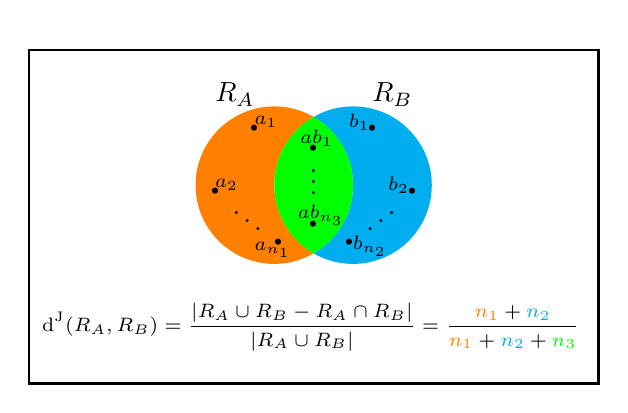
\begin{tikzpicture}[fill=gray]
% left hand
\begin{scope}
\clip (-2,-2) rectangle (2,2)
(1,0) circle (1);
\fill[orange] (0,0) circle (1);
\end{scope}
% right hand
\begin{scope}
\clip (-2,-2) rectangle (2,2)
(0,0) circle (1);
\fill[cyan] (1,0) circle (1);
\end{scope}
\begin{scope}
\clip (-2,-2) (0,0) circle (1);
\fill[green] (1,0) circle (1);
\end{scope}
% outline
%\draw (0,0) circle (1) (0,1)  node [text=black,above] {}
%(1,0) circle (1) (1,1)  node [text=black,above] {}
%(-3,-2.5) rectangle (4,2) node [text=black,above] {};
\node[text width=7cm,text height=4cm,line width=0.3mm,draw] at (0.5,-0.4) {};
\node [circle] (A) at (-0.5,1.15) {$R_A$};
\node [circle] (B) at (1.5,1.15) {$R_B$};
\node [text width=6.9cm] at (0.5,-1.8) (sets) {\scriptsize $\displaystyle \text{d}^\text{J}(R_A,R_B) = \frac{|R_A \cup R_B - R_A \cap R_B|}{|R_A \cup R_B|} = \displaystyle \frac{\textcolor{orange}{n_1} + \textcolor{cyan}{n_2}}{\textcolor{orange}{n_1} + \textcolor{cyan}{n_2} + \textcolor{green}{n_3}}$};
\node [text width=0.1cm] at (-0.3,0.7) (A1) {\huge $\cdot$};
\node [text width=0.1cm] at (-0.2,0.8) (vA1) {\scriptsize $a_1$};
\node [text width=0.1cm] at (-0.8,-0.1) (A2) {\huge $\cdot$};
\node [text width=0.1cm] at (-0.7,0.0) (vA2) {\scriptsize $a_2$};
\node [text width=0.1cm] at (-0.5,-0.35) (dots) {$\ddots$};
\node [text width=0.1cm] at (0,-0.75) (An1) {\huge $\cdot$};
\node [text width=0.1cm] at (-0.2,-0.82) (vAn1) {\scriptsize $a_{n_1}$};

\node [text width=0.1cm] at (0.45,0.45) (AB1) {\huge $\cdot$};
\node [text width=0.1cm] at (0.38,0.6) (vAB1) {\scriptsize $ab_1$};
\node [text width=0.1cm] at (0.5,0.15) (dots) {$\vdots$};
\node [text width=0.1cm] at (0.45,-0.52) (ABn3) {\huge $\cdot$};
\node [text width=0.1cm] at (0.35,-0.38) (vABn3) {\scriptsize $ab_{n_3}$};

\node [text width=0.1cm] at (1.2,0.7) (B1) {\huge $\cdot$};
\node [text width=0.1cm] at (1,0.8) (vB1) {\scriptsize $b_1$};
\node [text width=0.1cm] at (1.7,-0.1) (B2) {\huge $\cdot$};
\node [text width=0.1cm] at (1.5,0.0) (vB2) {\scriptsize $b_2$};
\node [text width=0.1cm] at (1.2,-0.35) (dots) {$\iddots$};
\node [text width=0.1cm] at (0.9,-0.75) (Bn2) {\huge $\cdot$};
\node [text width=0.1cm] at (1.05,-0.78) (vBn2) {\scriptsize $b_{n_2}$};

\end{tikzpicture}


\end{document}